\documentclass{beamer}
\usetheme{Antibes}
\usepackage{xcolor, colortbl}
\usepackage{algorithm}
\usepackage[noend]{algpseudocode}
\usepackage{textcomp}
\usepackage{listings}
\usepackage{hyperref}
\usepackage{alltt}
\usepackage{tikz}
\usepackage{framed}
\usepackage{marvosym}
\usepackage{wasysym}
\usepackage{marvosym}
\usepackage{crayola}
\usepackage{mathpartir}
\usepackage{tabularx}
\usepackage[belowskip=-15pt,aboveskip=0pt]{caption}
\usepackage[skins]{tcolorbox}
\usepackage{multicol}
\usetikzlibrary{positioning,shapes,arrows, backgrounds, fit, shadows, automata}
\usetikzlibrary{decorations.markings}
\setbeamertemplate{footline}[frame number]
\usefonttheme{serif}

\title[Sujit]{Parsing}
\author{Sujit Kumar Chakrabarti}
\institute{IIITB}
\date{}

\begin{document}
\maketitle
%
\definecolor{lightblue}{rgb}{0.8,0.93,1.0} % color values Red, Green, Blue
\definecolor{darkblue}{rgb}{0,0,0.5} % color values Red, Green, Blue
\definecolor{Blue}{rgb}{0,0,1.0} % color values Red, Green, Blue
\definecolor{darkgreen}{rgb}{0,0.7,0.2} % color values Red, Green, Blue
\definecolor{Red}{rgb}{1,0,0} % color values Red, Green, Blue
\definecolor{Pink}{rgb}{0.7,0,0.2}
\definecolor{links}{HTML}{2A1B81}
\definecolor{mydarkgreen}{HTML}{126215}
\definecolor{mychoco}{HTML}{5C3317}

\newcommand{\myheader}[1]{
	{\color{purple}
		\begin{Large}
			\begin{center}
				{#1}
			\end{center}
		\end{Large}
	}
}
\newcommand{\myminorheader}[1]{
	{\color{purple}
		\begin{large}
			{#1}
		\end{large}
	}
}

\newcommand{\myprod}[0]{\hspace{0.5cm}$\rightarrow$\hspace{0.5cm}}
\newcommand{\mychoice}[0]{\hspace{0.75cm}$|$\hspace{0.25cm}}
\newcommand{\myderiv}[0]{\hspace{0.5cm}$\Rightarrow$\hspace{0.5cm}}

\lstset{
	language = Caml,
	basicstyle = \ttfamily,
	stringstyle = \ttfamily,
	keywordstyle=\color{blue}\bfseries,
	identifierstyle=\color{mychoco},
	commentstyle=\color{darkgreen},
	frameround=tttt,
%	numbers=left,
	showstringspaces=false
}
\mathchardef\mhyphen="2D


\newsavebox{\redone}
\savebox{\redone}{
  
\begin{tikzpicture}
    \node(n1){\textbf{id}};
    \node(n2)[right of = n1]{*};
    \node(n3)[right of = n2]{\textbf{id}};
    
  \end{tikzpicture}
}

\newsavebox{\redtwo}
\savebox{\redtwo}{
  \begin{tikzpicture}
    \node(n1){$F$};
    \node(n2)[right of = n1]{*};
    \node(n3)[right of = n2]{\textbf{id}};
    \node(n4)[below of = n1]{\textbf{id}};
  \path 
    		(n1) edge node {}  (n4)
    ; 
  \end{tikzpicture}
}

\newsavebox{\redthree}
\savebox{\redthree}{
  \begin{tikzpicture}
    \node(n1){$T$};
    \node(n2)[right of = n1]{*};
    \node(n3)[right of = n2]{\textbf{id}};
    \node(n4)[below of = n1]{$F$};
    \node(n5)[below of = n4]{\textbf{id}};
  \path 
    		(n1) edge node {}  (n4)
    		(n4) edge node {}  (n5)
    ; 
  \end{tikzpicture}
}

\newsavebox{\redfour}
\savebox{\redfour}{
  \begin{tikzpicture}
    \node(n1){$T$};
    \node(n2)[right of = n1]{*};
    \node(n3)[right of = n2]{$F$};
    \node(n4)[below of = n1]{$F$};
    \node(n5)[below of = n4]{\textbf{id}};
    \node(n6)[below of = n3]{\textbf{id}};
  \path 
    		(n1) edge node {}  (n4)
    		(n4) edge node {}  (n5)
    		(n3) edge node {}  (n6)
    ; 
  \end{tikzpicture}
}

\newsavebox{\redfive}
\savebox{\redfive}{
  \begin{tikzpicture}
    \node(n1){$T$};
    \node(n2)[right of = n1]{*};
    \node(n3)[right of = n2]{$F$};
    \node(n4)[below of = n1]{$F$};
    \node(n5)[below of = n4]{\textbf{id}};
    \node(n6)[below of = n3]{\textbf{id}};
    \node(n7)[above of = n2]{$T$};

  \path 
    		(n1) edge node {}  (n4)
    		(n4) edge node {}  (n5)
    		(n3) edge node {}  (n6)
    		(n7) edge node {}  (n1)
    		(n7) edge node {}  (n2)
    		(n7) edge node {}  (n3)
    ; 
  \end{tikzpicture}
}

\newsavebox{\redsix}
\savebox{\redsix}{
  \begin{tikzpicture}
    \node(n1){$T$};
    \node(n2)[right of = n1]{*};
    \node(n3)[right of = n2]{$F$};
    \node(n4)[below of = n1]{$F$};
    \node(n5)[below of = n4]{\textbf{id}};
    \node(n6)[below of = n3]{\textbf{id}};
    \node(n7)[above of = n2]{$T$};
    \node(n8)[above of = n7]{$E$};

  \path 
    		(n1) edge node {}  (n4)
    		(n4) edge node {}  (n5)
    		(n3) edge node {}  (n6)
    		(n7) edge node {}  (n1)
    		(n7) edge node {}  (n2)
    		(n7) edge node {}  (n3)
    		(n8) edge node {}  (n7)
    ; 
  \end{tikzpicture}
}

% frame begin %%%%%%%%%%%%%%%%%%%%%%%%
\begin{frame}{Bottom-up Parsing}
{Example}

\begin{scriptsize}
\begin{tabular}{c @{\hspace{1cm}} c}

\begin{minipage}{0.3\textwidth}

\myminorheader{Grammar}
\begin{tabular}{l @{} c @{} l}
$E$     & {\myprod}   & $E$ + $T | T$         \\
$T$     & {\myprod}   & $T * F | F$   \\
$F$     & {\myprod}   & ($E$)     \\
        & {\mychoice} & \textbf{id}
\end{tabular}
\vspace{0.5cm}

\myminorheader{Input: }1 * 2
\end{minipage}

&
\begin{minipage}{0.6\textwidth}
\pause

\begin{center}
\resizebox{0.9\textwidth}{!}{%
\begin{tikzpicture}[auto,
    -,
  %  shorten >=2pt,
    >=stealth,
    node distance=0.5cm,
    bb/.style={%
      rectangle, draw=black, very thick, fill=white,
      text ragged, minimum height=2em, inner sep=6pt, align=center
    },
    inv/.style={%
      rectangle, draw=none, fill=white,
      text ragged, minimum height=2em, inner sep=6pt, align=center
    }
]

    \node(1) at (0, 1)  {\usebox{\redone}};
	\pause
    \node(2) at (5, 0.5)  {\usebox{\redtwo}};
	\pause
    \node(3) at (10, 0)  {\usebox{\redthree}};
	\pause
    \node(4) at (0, -3)  {\usebox{\redfour}};
	\pause
    \node(5) at (5, -3.5)  {\usebox{\redfive}};
	\pause
    \node(6) at (10, -4)  {\usebox{\redsix}};

  \end{tikzpicture}
}
\end{center}
\end{minipage}
\\
\end{tabular}
\end{scriptsize}

\end{frame}
% frame end %%%%%%%%%%%%%%%%%%%%%%%%

% frame begin %%%%%%%%%%%%%%%%%%%%%%%%
\begin{frame}{Bottom-up Parsing}
{Example}

\begin{center}
\resizebox{0.7\textwidth}{!}{%
\begin{tikzpicture}[auto,
    -,
  %  shorten >=2pt,
    >=stealth,
    node distance=0.5cm,
    bb/.style={%
      rectangle, draw=black, very thick, fill=white,
      text ragged, minimum height=2em, inner sep=6pt, align=center
    },
    inv/.style={%
      rectangle, draw=none, fill=white,
      text ragged, minimum height=2em, inner sep=6pt, align=center
    }
]

    \node(1) at (0, 1)  {\usebox{\redone}};
    \node(2) at (5, 0.5)  {\usebox{\redtwo}};
    \node(3) at (10, 0)  {\usebox{\redthree}};
    \node(4) at (0, -3)  {\usebox{\redfour}};
    \node(5) at (5, -3.5)  {\usebox{\redfive}};
    \node(6) at (10, -4)  {\usebox{\redsix}};

  \end{tikzpicture}
}

\end{center}

\myminorheader{Derivation}: \\
$E \Rightarrow T\Rightarrow T * F \Rightarrow T * id \Rightarrow F * id \Rightarrow id * id$

\begin{enumerate}
	\pause
	\item Rightmost derivation
	\pause
	\item Reverse rightmost derivation -- \emph{Reduction}
\end{enumerate}
\end{frame}
% frame end %%%%%%%%%%%%%%%%%%%%%%%%

% frame begin %%%%%%%%%%%%%%%%%%%%%%%%
\begin{frame}{Bottom-up Parsing}
{Right Sentential Form}
\begin{itemize}
	\item \textbf{Right Sentential Form.} Strings of grammar symbols that occur anytime during a rightmost derivation from a grammar $G$
	\item All \emph{frontiers} during a bottom-up parse are right sentential forms.  
\end{itemize}
\end{frame}
% frame end %%%%%%%%%%%%%%%%%%%%%%%%

% frame begin %%%%%%%%%%%%%%%%%%%%%%%%
\begin{frame}{Bottom-up Parsing}
{Handle}
\begin{itemize}
	\item \textbf{Handle.} A sub-string of a right-sentential form that appears as a right hand side of a grammar production, and which can be used to reduce the string to its \emph{previous} right-sentential form
	\item $S \stackrel{*}{\Rightarrow} \alpha A w \Rightarrow \alpha \beta w$ with a production $A \rightarrow \beta$, then $A \rightarrow \beta$ is a handle.
	\pause
	\item Bottom-up parsing can be viewed as the process of locating a handle in the $n$-th right-sentential form of $S$, and replacing that with the LHS of the production to get the $(n - 1)$th right-sentential form. 
\end{itemize}
\end{frame}
% frame end %%%%%%%%%%%%%%%%%%%%%%%%

% frame begin %%%%%%%%%%%%%%%%%%%%%%%%
\begin{frame}{Shift-Reduce Parsing}
\begin{center}
\begin{tabular}{c @{} c @{} c}
\textbf{Stack} &              & \textbf{Input} \\
\hline
$\$$           &              & $w\$$ \\
\pause
               & $\downarrow$ &       \\
$\$S$          &              & $\$$
\end{tabular}
\end{center}

\myminorheader{Example:}

\begin{scriptsize}
\begin{center}
\begin{tabular}{l | r | l}
\textbf{Stack} & \textbf{Input} & \textbf{Action} \\
\hline
$\$$                & $\textbf{id}_1 * \textbf{id}_2\$$ & shift                                       \\
\pause
$\$\textbf{id}_1$   & $* \textbf{id}_2\$$               & reduce by $F \rightarrow \textbf{id}$       \\
\pause
$\$F$               & $* \textbf{id}_2\$$               & reduce by $T \rightarrow F$                 \\
\pause
$\$T$               & $* \textbf{id}_2\$$               & shift                                       \\
\pause
$\$T*$              & $\textbf{id}_2\$$                 & shift                                       \\
\pause
$\$T*\textbf{id}_2$ & $\$$                              & reduce by $F \rightarrow \textbf{id}$       \\
\pause
$\$T*F$             & $\$$                              & reduce by $T \rightarrow + T*F$             \\
\pause
$\$T$               & $\$$                              & reduce by $E \rightarrow T$                 \\
\pause
$\$E$               & $\$$                              &                                             \\
\end{tabular}
\end{center}
\end{scriptsize}

\end{frame}
% frame end %%%%%%%%%%%%%%%%%%%%%%%%

% frame begin %%%%%%%%%%%%%%%%%%%%%%%%
\begin{frame}{Shift-Reduce Parsing}
{Parser Actions}
\begin{enumerate}
	\item \textbf{Shift:} Shift the next input symbol onto the stack.
	\item \textbf{Reduce: } Reduce a contiguous portion of the stack content including the top-of-stack by the LHS of an appropriate grammar production.
	\pause
	\item \textbf{Accept: }Declare success.
	\item \textbf{Error: }Discover a syntax error.
\end{enumerate}
\end{frame}
% frame end %%%%%%%%%%%%%%%%%%%%%%%%

% frame begin %%%%%%%%%%%%%%%%%%%%%%%%
\begin{frame}{Shift-Reduce Parsing}
{Reductions happen only at the top of the stack}
\begin{enumerate}
	\item $S \substack{* \\ \Rightarrow \\ rm} \alpha A z \Rightarrow \alpha \beta Byz \substack{\\ \Rightarrow \\ rm} \alpha \beta \gamma yz$
	\item $S \substack{* \\ \Rightarrow \\ rm} \alpha B x A z \Rightarrow \alpha Bxyz \substack{\\ \Rightarrow \\ rm} \alpha \gamma x y z$ 
\end{enumerate}

\pause
Derivations to the left happen later. Reductions to the left happen earlier.
\end{frame}
% frame end %%%%%%%%%%%%%%%%%%%%%%%%

% frame begin %%%%%%%%%%%%%%%%%%%%%%%%
\begin{frame}{Shift-Reduce Parsing}
{Condition for a Successful Parse}
\pause
\myminorheader{Viable Prefix} \\
A prefix of a right-sentential form.
\pause

\vspace{1cm}
\myminorheader{Conflicts}
\begin{enumerate}
	\item \textbf{Shift-Reduce}
	\item \textbf{Reduce-Reduce}
\end{enumerate}
\end{frame}
% frame end %%%%%%%%%%%%%%%%%%%%%%%%


% frame begin %%%%%%%%%%%%%%%%%%%%%%%%
\begin{frame}{Shift-Reduce Parsing}
{Conflicts}
\myminorheader{Example} \\
\begin{tabular}{l @{} c @{} l}
$stmt$     & {\myprod}   & if $expr$ then $stmt$             \\
           & {\mychoice} & if $expr$ then $stmt$ else $stmt$ \\
           & {\mychoice} & other
\end{tabular}

\end{frame}
% frame end %%%%%%%%%%%%%%%%%%%%%%%%

\newsavebox{\dangone}
\savebox{\dangone}{
  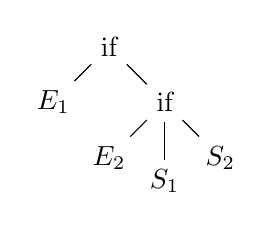
\begin{tikzpicture}
    \node(n1){if};
    \node(n2)[below left of = n1]{$E_1$};
    \node(n3)[below right of = n1]{if};
    \node(n4)[below left of = n3]{$E_2$};
    \node(n5)[below of = n3]{$S_1$};
    \node(n6)[below right of = n3]{$S_2$};

  \path 
    		(n1) edge node {}  (n2)
    		(n1) edge node {}  (n3)
    		(n3) edge node {}  (n4)
    		(n3) edge node {}  (n5)
    		(n3) edge node {}  (n6)
    ; 
  \end{tikzpicture}
}

\newsavebox{\dangtwo}
\savebox{\dangtwo}{
  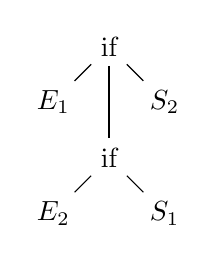
\begin{tikzpicture}
    \node(n1){if};
    \node(n2)[below left of = n1]{$E_1$};
    \node(n3)[below right of = n2]{if};
    \node(n4)[below left of = n3]{$E_2$};
    \node(n5)[below right of = n3]{$S_1$};
    \node(n6)[below right of = n1]{$S_2$};

  \path 
    		(n1) edge node {}  (n2)
    		(n1) edge node {}  (n3)
    		(n1) edge node {}  (n6)
    		(n3) edge node {}  (n4)
    		(n3) edge node {}  (n5)
    ; 
  \end{tikzpicture}
}

% frame begin %%%%%%%%%%%%%%%%%%%%%%%%
\begin{frame}{Bottom-up Parsing}
{Conflict -- Example}

\textbf{input:} if $E_1$ then if $E_2$ then $S_1$ else $S_2$

\pause
\begin{center}
\resizebox{0.7\textwidth}{!}{%
\begin{tikzpicture}[auto,
    -,
  %  shorten >=2pt,
    >=stealth,
    node distance=0.5cm,
    bb/.style={%
      rectangle, draw=black, very thick, fill=white,
      text ragged, minimum height=2em, inner sep=6pt, align=center
    },
    inv/.style={%
      rectangle, draw=none, fill=white,
      text ragged, minimum height=2em, inner sep=6pt, align=center
    }
]

    \node(1) at (0, 0)  {\usebox{\dangone}};

    \node(1) at (3, 0)  {\usebox{\dangtwo}};

  \end{tikzpicture}
}

\pause
\begin{itemize}
	\item \underline{if $E_1$ then \underline{if $E_2$ then $S_1$} else $S_2$}
	\item \underline{if $E_1$ then \underline{if $E_2$ then $S_1$ else $S_2$}}
\end{itemize}
\end{center}

\end{frame}
% frame end %%%%%%%%%%%%%%%%%%%%%%%%

% frame begin %%%%%%%%%%%%%%%%%%%%%%%%
\begin{frame}{Bottom-up Parsing}
{LR Parsing}


\myminorheader{Properties}
\begin{itemize}
	\item Table driven
	\item LR grammars
\end{itemize}

\pause
\myminorheader{Advantages}
\begin{itemize}
	\item LR grammars are quite general.
	\item Syntax errors are detected early.
	\item $LR(k) \supset LL(k)$
\end{itemize}

\end{frame}
% frame end %%%%%%%%%%%%%%%%%%%%%%%%

% frame begin %%%%%%%%%%%%%%%%%%%%%%%%
\begin{frame}{Bottom-up Parsing}
{LR Parsing}

\myminorheader{Properties}
\begin{itemize}
	\item Table driven
	\item LR grammars
\end{itemize}

\myminorheader{Advantages}
\begin{itemize}
	\item LR grammars are quite general.
	\item Syntax errors are detected early.
	\item $LR(k) \supset LL(k)$
\end{itemize}

\end{frame}
% frame end %%%%%%%%%%%%%%%%%%%%%%%%

% frame begin %%%%%%%%%%%%%%%%%%%%%%%%
\begin{frame}{SLR Parsing}
{Parser Architecture}
\begin{center}
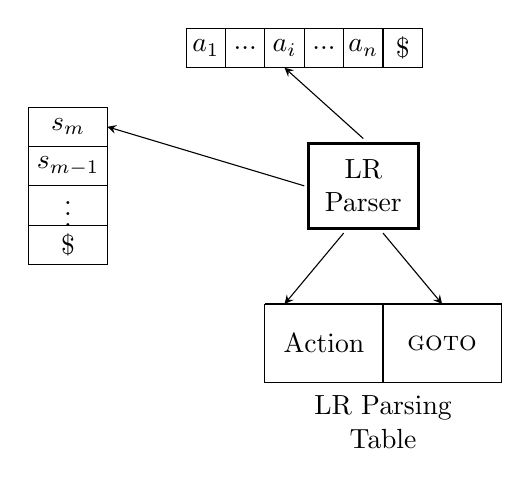
\begin{tikzpicture}[auto,
    -,
  %  shorten >=2pt,
    >=stealth,
    node distance=0.5cm,
    bb/.style={%
      rectangle, draw=black, very thick, fill=white,
      text ragged, minimum height=2em, inner sep=6pt, align=center
    },
    inv/.style={%
      rectangle, draw=none, fill=white,
      text ragged, minimum height=2em, inner sep=6pt, align=center
    }
]
% input string
\draw (0,-1) -- ++(3cm,0) -- ++(0,-0.5cm) -- ++(-3cm,0) -- ++(0,0.5cm);
\foreach \i in {1,...,5}
  \draw (\i*0.5cm,-1) -- +(0,-0.5cm);
\node at (0.25,-1.25cm) {$a_1$};
\node at (0.75,-1.25cm) {$...$};
\node at (1.25,-1.25cm) {$a_i$};
\node at (1.75,-1.25cm) {$...$};
\node at (2.25,-1.25cm) {$a_n$};
\node at (2.75,-1.25cm) {$\$$};

% stack
\draw (-2,-2) -- ++(1cm, 0) -- ++(0,-2cm) -- ++(-1cm,0) -- ++(0,2cm);
\foreach \i in {1,...,3}
  \draw (-2cm,-2cm-\i*0.5cm) -- +(1cm,0);
\node at (-1.5,-2.25cm) {$s_m$};
\node at (-1.5,-2.75cm) {$s_{m-1}$};
\node at (-1.5,-3.25cm) {$\vdots$};
\node at (-1.5,-3.75cm) {$\$$};

\node[bb](1) at (2.25,-3.00cm) {LR \\ Parser};

% LR Parsing Table
\draw (1,-4.5) -- ++(3cm,0) -- ++(0,-1cm) -- ++(-3cm,0) -- ++(0,1cm);
  \draw (2.5,-4.5) -- +(0,-1cm);

\node at (1.75, -5) {Action};
\node at (3.25, -5) {\textsc{goto}};

\node[align = center] at (2.5, -6) {LR Parsing \\ Table};

\draw[->] (2,-3.6) -- +(-0.75,-0.9); % Predictive Parser -> Transition Table (Action)
\draw[->] (2.5,-3.6) -- +(0.75,-0.9); % Predictive Parser -> Transition Table (goto)
\draw[->] (2.25,-2.4) -- +(-1,0.9); % Predictive Parser -> Input Queue
\draw[->] (1.5,-3) -- +(-2.5,0.75); % Predictive Parser -> Stack
\end{tikzpicture}
\end{center}
\end{frame}
% frame end %%%%%%%%%%%%%%%%%%%%%%%%

\end{document}
